%% ====================================================================
%% talk_ALCIRCC5.tex -- work presentation (~35 slides, 16:9, metropolis)
%%
%% "Can Agentic AI Settle a 20-Year-Old Open Problem?"
%% Based on papers/overview_arxiv.tex (the frozen arXiv candidate).
%% Build:  pdflatex talk_ALCIRCC5.tex  (twice, for the progress bar)
%% ====================================================================
\documentclass[aspectratio=169,11pt]{beamer}

\usetheme[progressbar=frametitle]{metropolis}
\metroset{numbering=fraction, sectionpage=none}

\usepackage[T1]{fontenc}
\usepackage{booktabs}
\usepackage{colortbl}
\usepackage{tikz}
\usetikzlibrary{positioning,arrows.meta,calc}
\newcommand{\xmark}{\textcolor{openc}{\raisebox{.5pt}{$\times$}}}

%% ---- palette -------------------------------------------------------
\definecolor{petrol}{RGB}{14,110,119}
\definecolor{warm}{RGB}{176,90,20}
\definecolor{good}{RGB}{46,125,79}
\definecolor{openc}{RGB}{160,109,16}
\setbeamercolor{progress bar}{fg=petrol}
\setbeamercolor{alerted text}{fg=warm}
\setbeamercolor{frametitle}{bg=black!85}

%% ---- macros (mirroring the paper) ----------------------------------
\newcommand{\ALCIRCC}[1]{\mathcal{ALCI}_{\mathrm{RCC#1}}}
\newcommand{\ALCI}{\ensuremath{\mathcal{ALCI}}}
\newcommand{\DR}{\mathsf{DR}}
\newcommand{\PO}{\mathsf{PO}}
\newcommand{\PP}{\mathsf{PP}}
\newcommand{\PPI}{\mathsf{PPI}}
\newcommand{\EQ}{\mathsf{EQ}}
\newcommand{\comp}{\ensuremath{\mathsf{comp}}}
\newcommand{\EXPTIME}{\textsc{ExpTime}}
\newcommand{\PSPACE}{\textsc{PSpace}}
\newcommand{\cl}{\ensuremath{\mathsf{cl}}}
\newcommand{\statuslabel}{\textcolor{openc}{\textbf{strongly supported, \emph{not} certified}}}

%% two-circle pictograms for the five relations
\newcommand{\picDR}{
\begin{tikzpicture}[scale=.5,baseline=-2pt]
  \draw[thick,petrol] (0,0) circle (.30); \draw[thick,warm] (.85,0) circle (.30);
\end{tikzpicture}}
\newcommand{\picPO}{
\begin{tikzpicture}[scale=.5,baseline=-2pt]
  \draw[thick,petrol] (0,0) circle (.30); \draw[thick,warm] (.38,0) circle (.30);
\end{tikzpicture}}
\newcommand{\picEQ}{
\begin{tikzpicture}[scale=.5,baseline=-2pt]
  \draw[thick,petrol] (0,0) circle (.30); \draw[thick,warm,dashed] (0,0) circle (.24);
\end{tikzpicture}}
\newcommand{\picPP}{
\begin{tikzpicture}[scale=.5,baseline=-2pt]
  \draw[thick,warm] (0,0) circle (.32); \draw[thick,petrol] (-.09,-.05) circle (.16);
\end{tikzpicture}}
\newcommand{\picPPI}{
\begin{tikzpicture}[scale=.5,baseline=-2pt]
  \draw[thick,petrol] (0,0) circle (.32); \draw[thick,warm] (.09,-.05) circle (.16);
\end{tikzpicture}}

\title{Can Agentic AI Settle a\\ 20-Year-Old Open Problem?}
\subtitle{The decidability of $\ALCIRCC{5}$ --- a machine-checked campaign}
\author{Michael Wessel\\[2pt]
  {\small with AI assistants: Claude (Anthropic) and GPT-5.4/5.5/5.6~Pro (OpenAI)}}
\date{July 2026}

\begin{document}

%% ==================================================================== 1
\maketitle

%% ==================================================================== 2
\begin{frame}{The one-slide version}
\begin{itemize}
  \item In 2002/2003 I defined a family of \alert{spatial description logics}
        and left their central decidability question \alert{open}. It still is.
  \item In 2026 I directed a \alert{four-month AI campaign} on it:
        two frontier models, adversarial review, machine verification.
  \item The question is \alert{not settled}. But it is now \emph{reduced} ---
        honestly and partly kernel-checked --- to \alert{one well-posed lemma},
        with a decidable fragment, a certified normal form, a working reasoner,
        and an exact arithmetical address ($\Pi^0_1$) along the way.
\end{itemize}
\vfill
\begin{block}{How to read everything in this talk}
  The mathematics was produced by AI assistants and is
  \emph{unverified by human experts}. Standing label: \statuslabel{}\,---\,%
  except the parts checked by the \alert{Lean~4 kernel}, which are
  machine-verified (but still human-unreviewed).
\end{block}
\end{frame}

%% ==================================================================== 3
\section{The problem}
\begin{frame}{Five ways two regions can relate (RCC5)}
\begin{center}
\renewcommand{\arraystretch}{1.3}
\begin{tabular}{ccccc}
  \picDR & \picPO & \picEQ & \picPP & \picPPI\\[4pt]
  $\DR$ & $\PO$ & $\EQ$ & $\PP$ & $\PPI$\\
  disjoint & partial overlap & equal & proper part & proper superpart
\end{tabular}
\end{center}
\vfill
\begin{itemize}
  \item Every pair of regions stands in \alert{exactly one} of these five relations.
  \item \emph{Jointly exhaustive, pairwise disjoint} --- the classic
        qualitative spatial calculus (a coarser cousin of RCC8).
  \item Think GIS, layout, biology, any ``what contains / touches what''
        domain --- \alert{no coordinates required}.
\end{itemize}
\end{frame}

%% ==================================================================== 4
\begin{frame}{Reasoning without geometry: the composition table}
If I know $x \mathrel{R} y$ and $y \mathrel{S} z$, what can $x \mathrel{?} z$ be?
\begin{center}
\begin{tabular}{lll}
  \toprule
  known & known & forced / allowed\\
  \midrule
  $x\,\PP\,y$ & $y\,\PP\,z$ & $x\,\PP\,z$ \hfill (\emph{forced}: parts of parts are parts)\\
  $x\,\PP\,y$ & $y\,\DR\,z$ & $x\,\DR\,z$ \hfill (\emph{forced}: inside something disjoint)\\
  $x\,\DR\,y$ & $y\,\DR\,z$ & anything at all \hfill (\emph{free}: 5 options)\\
  \bottomrule
\end{tabular}
\end{center}
\vfill
\begin{itemize}
  \item All 25 cells form the \alert{composition table} --- pure algebra,
        derived once from set semantics, then used forever.
  \item \alert{Abstract semantics}: a ``model'' is any relation assignment
        closed under this table --- \emph{space itself has left the building}.
  \item Every probe in this project re-derives the table from scratch,
        so the algebra can never silently drift.
\end{itemize}
\end{frame}

%% ==================================================================== 5
\begin{frame}{A description logic: you write definitions and facts}
A \alert{TBox} is a set of concept \emph{definitions}, built from properties
and \alert{quantified spatial relations}:
\begin{align*}
  \textsf{CityAtRiver} &\;\equiv\; \textsf{City} \sqcap \exists\PO.\,\textsf{River}
      && \text{\small a city \emph{overlapping} a river}\\
  \textsf{GermanCity} &\;\equiv\; \textsf{City} \sqcap
      \forall\PP.(\neg\textsf{Country}\sqcup\textsf{Germany})
      && \text{\small a city in \emph{no country but} Germany}
\end{align*}
\vfill
Then we \alert{assert} a few primitive facts --- and nothing more:
\begin{align*}
  \textsf{Hamburg} &\;\sqsubseteq\; \textsf{City} \sqcap \exists\PO.\,\textsf{Alster}
      \qquad\text{\small(a city, overlapping the Alster)}\\
  \textsf{Alster} &\;\sqsubseteq\; \textsf{River} \sqcap \exists\PP.\textsf{Germany}
      \sqcap \forall\PO.\neg\textsf{Country}
      \sqcap \forall\PP.(\neg\textsf{Country}\sqcup\textsf{Germany})
\end{align*}
\vfill
{\small Note what we did \emph{not} say: that Hamburg is a
\textsf{GermanCity}, or a \textsf{CityAtRiver}.}
\end{frame}

%% ==================================================================== 5b
\begin{frame}{\dots\ and the reasoner \emph{infers} the classification}
We never \emph{asserted} that Hamburg is a \textsf{GermanCity} or a
\textsf{CityAtRiver} --- the \alert{reasoner derives both}.
\smallskip

\textbf{City at a river} (immediate):
\[
  \textsf{Hamburg}\ \PO\ \textsf{Alster}
  \;\wedge\; \textsf{Alster}\sqsubseteq\textsf{River}
  \;\Longrightarrow\;
  \textsf{Hamburg}\sqsubseteq\textsf{City}\sqcap\exists\PO.\textsf{River}
  = \textsf{CityAtRiver}.
\]

\textbf{German city} --- needs the \alert{composition table}. For any country
$c$ with $\textsf{Hamburg}\ \PP\ c$:
\begin{itemize}\small
  \item $\textsf{Alster}\ \PO\ \textsf{Hamburg}\ \PP\ c
        \;\Rightarrow\; \textsf{Alster}\,\{\PO,\PP\}\,c$
        \hfill $\comp(\PO,\PP)=\{\PO,\PP\}$
  \item Alster overlaps no country ($\forall\PO.\neg\textsf{Country}$)
        $\;\Rightarrow\; \textsf{Alster}\ \PP\ c$
  \item Alster's only country-superpart is Germany
        $\;\Rightarrow\; c=\textsf{Germany}$
\end{itemize}
So Hamburg \emph{is} a German city --- and every hidden fact reduces to
\alert{concept satisfiability}: $C\sqsubseteq D$ iff $C\sqcap\neg D$ unsat.
\end{frame}

%% ==================================================================== 6
\begin{frame}{$\ALCIRCC{5}$: the spatial relations \emph{become} the roles}
\begin{columns}[T]
\column{.55\textwidth}
  \textbf{The logic} (Wessel 2002/2003):
  \begin{itemize}
    \item $\ALCI$ = the basic DL with inverse roles;
    \item roles = the five RCC5 relations themselves;
    \item the composition table is enforced \alert{globally};
    \item $\EQ$ = identity (\emph{strong} semantics).
  \end{itemize}
  \medskip
  So one can say things like
  \[
    \forall\PP.\,\neg\textsf{Lake} \qquad \exists\DR.\,\textsf{Reserve}
  \]
  ``no part is a lake'', ``disjoint from some reserve''.
\column{.42\textwidth}
  \begin{block}{Why this is different}
    Concrete-domain DLs constrain spatial \emph{attributes} of objects.
    Here the relations are \emph{first-class roles}: one can
    \alert{quantify over them}. None of the known concrete-domain
    decidability results apply.
  \end{block}
\end{columns}
\end{frame}

%% ==================================================================== 7
\begin{frame}{Why the standard toolbox dies on contact}
Every pair of elements carries a relation $\Rightarrow$ a model is a
\alert{complete labelled graph}, never a tree.
\vfill
\begin{columns}[T]
\column{.31\textwidth}
\begin{center}\textbf{no tree models}\end{center}
Blocking/unravelling --- the workhorse of DL decidability --- has no tree
to work on.
\column{.31\textwidth}
\begin{center}\textbf{no finite models}\end{center}
$\exists\PPI.\top \sqcap \forall\PPI.\exists\PPI.\top$ forces an infinite
ascending part-of tower.
\column{.31\textwidth}
\begin{center}\textbf{nondeterministic table}\end{center}
Most cells allow several outcomes --- composition \emph{constrains} but
rarely \emph{determines}.
\end{columns}
\vfill
\begin{center}
\alert{Creating one new element forces relations to \emph{every} existing
element} --- and a dormant $\forall$ anywhere may wake up because of it.
\end{center}
\end{frame}

%% ==================================================================== 8
\begin{frame}{The landscape: open exactly at the top}
\begin{center}
\small
\begin{tabular}{lll}
\toprule
Logic & Relations & Concept satisfiability\\
\midrule
$\ALCIRCC{1}$ & $\{\mathsf{SR}\}$ & decidable ($\equiv$ S5)\\
$\ALCIRCC{2}$ & $\{\DR,\mathsf{O}\}$ & decidable\\
$\ALCIRCC{3}$ & $\{\DR,\mathsf{ONE},\EQ\}$ & decidable \hfill {\footnotesize(via two-variable FO!)}\\
\rowcolor{petrol!12}
$\ALCIRCC{5}$, $\forall\PO$-free & RCC5 w/o $\forall\PO$ & \textbf{decidable} \hfill {\footnotesize(this project)}\\
\rowcolor{openc!15}
$\ALCIRCC{5}$ & all five & \textbf{open}; \PSPACE-hard\\
\rowcolor{openc!15}
$\ALCIRCC{8}$ & eight RCC8 rel. & \textbf{open}; \EXPTIME-hard\\
\bottomrule
\end{tabular}
\end{center}
\vfill
Lutz \& Wolter 2006, after proving the \emph{topological} cousins undecidable:
\begin{quote}
``Perhaps the most interesting candidate is $L_{RCC5}(RS)$ [\,=\,$\ALCIRCC{5}$]
\dots\ to which the reduction exhibited in Section 8 does not apply.''
\end{quote}
Recognized open by the leading experts --- for \alert{twenty years}.
\end{frame}

%% ==================================================================== 9
\section{Why it is hard: the two axes}
\begin{frame}{One logic, two completely different axes}
\begin{center}
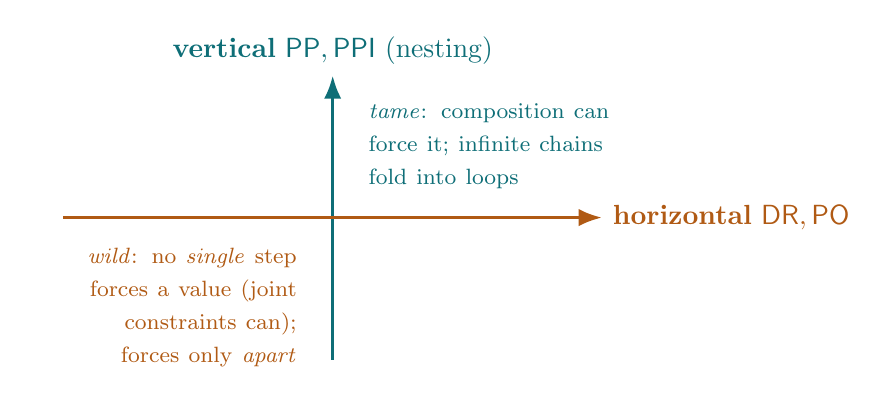
\begin{tikzpicture}[scale=.95]
  \draw[-{Latex},very thick,petrol] (0,-1.9) -- (0,1.9)
     node[above] {\textbf{vertical} $\PP,\PPI$ (nesting)};
  \draw[-{Latex},very thick,warm] (-3.6,0) -- (3.6,0)
     node[right] {\textbf{horizontal} $\DR,\PO$};
  \node[petrol,align=left,anchor=west,text width=3.3cm] at (.35,.95)
     {\footnotesize\emph{tame}: composition can force it; infinite chains fold into loops};
  \node[warm,align=right,anchor=east,text width=3.3cm] at (-.35,-1.2)
     {\footnotesize\emph{wild}: no \emph{single} step forces a value (joint constraints can); forces only \emph{apart}};
\end{tikzpicture}
\end{center}
\vfill
\begin{itemize}
  \item Depth (nesting) is \alert{never the problem} --- ordinary modal-logic folding handles it.
  \item Everything hard lives in \alert{horizontal crowds}: many pairwise-distinct
        neighbours that no finite summary seems to capture.
\end{itemize}
\end{frame}

%% ==================================================================== 10
\begin{frame}{The asymmetry, made precise (machine-verified)}
\textbf{No \emph{single} step forces a horizontal value.} Of the 16
compositions of proper relations, exactly \alert{four} return a single value:
\begin{center}
\resizebox{0.72\textwidth}{!}{$\comp(\DR,\PPI)=\comp(\PP,\DR)=\{\DR\},\quad
\comp(\PP,\PP)=\{\PP\},\quad \comp(\PPI,\PPI)=\{\PPI\}$}
\end{center}
--- every one runs through $\PP/\PPI$; no single cell yields $\{\PO\}$.
\alert{But the \emph{intersection} of several can force $\PO$}
($\comp(\DR,\PO)\cap\comp(\PPI,\PO)=\{\PO\}$) --- so ``shadow'' is joint
closure, not single-path.
\medskip

\textbf{Disjointness is half-deterministic.}
\begin{center}\small
\textcolor{good}{\textbf{downward}}: $x\,\DR\,y \Rightarrow$ every part of $x$
is $\DR$ from every part of $y$\\[2pt]
\textcolor{openc}{\textbf{upward}}: a superpart of $x$ may be $\DR$, $\PO$, or
$\PPI$ to $y$ --- \alert{free}
\end{center}
\medskip

So one high $\DR$ edge dispatches an \emph{arbitrarily wide} crowd of
disjointnesses below it, for free. What resists: $\PO$, and the upward direction.
\end{frame}

%% ==================================================================== 11
\begin{frame}{Shadows, live width, and the one property that matters}
\begin{itemize}
  \item An edge is a \alert{shadow} if composition already forces it from
        edges you have --- it costs a decision procedure \emph{nothing}.
  \item The \alert{live width} of an interface = the number of
        \emph{non-shadow} edges there: the genuine branching that must be recorded.
\end{itemize}
\vfill
\begin{block}{Property F6 (the keystone of everything)}
  Is the live width of models bounded by a computable function of the
  input concept?
\end{block}
\vfill
\begin{center}
  \textbf{If yes} $\Rightarrow$ finite certificate space $\Rightarrow$
  \alert{satisfiability is decidable}.
\end{center}
\end{frame}

%% ==================================================================== 12
\begin{frame}{The knife's edge: one fact, two futures}
\begin{center}
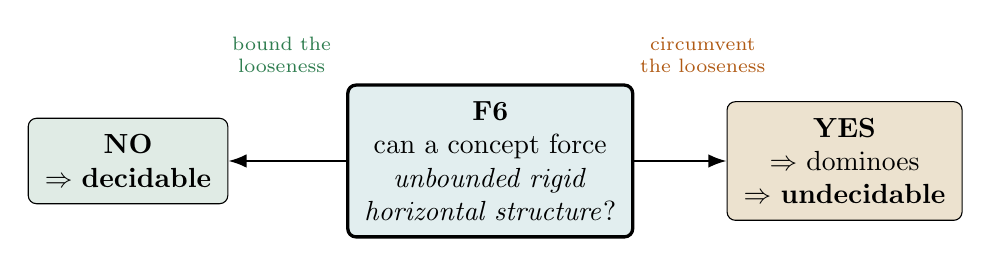
\begin{tikzpicture}[
  box/.style={draw, rounded corners=3pt, align=center, inner sep=6pt},
  lab/.style={font=\scriptsize, align=center}]
  \node[box, fill=petrol!12, very thick] (f6) at (0,0)
    {\textbf{F6}\\ can a concept force\\ \emph{unbounded rigid}\\ \emph{horizontal structure}?};
  \node[box, fill=good!15] (dec) at (-4.6,0) {\textbf{NO}\\ $\Rightarrow$ \textbf{decidable}};
  \node[box, fill=openc!20] (und) at (4.5,0) {\textbf{YES}\\ $\Rightarrow$ dominoes\\ $\Rightarrow$ \textbf{undecidable}};
  \draw[-{Latex}, thick] (f6) -- (dec);
  \draw[-{Latex}, thick] (f6) -- (und);
  \node[lab, good] at (-2.65,1.35) {bound the\\ looseness};
  \node[lab, warm] at (2.7,1.35) {circumvent\\ the looseness};
\end{tikzpicture}
\end{center}
\vfill
The \emph{same} looseness of the composition table blocks \alert{both}
proofs. That is \emph{why} neither direction has been settled in twenty
years --- it is one question seen from two sides.
\end{frame}

%% ==================================================================== 13
\section{Why undecidability keeps failing}
\begin{frame}{The standard weapon needs a rigid grid}
\begin{itemize}
  \item Classic undecidability proofs encode \alert{domino tilings} of
        $\mathbb{N}\times\mathbb{N}$: build a grid, force tile constraints,
        reduce the halting problem.
  \item The crux is \alert{rigidity}: going \emph{east then north} must land on
        \emph{exactly the same cell} as \emph{north then east}
        ($R_X \circ R_Y = R_Y \circ R_X$, the ``coincidence condition'').
  \item Every known route into $\ALCIRCC{}$ needs a feature it does not have:
        number restrictions, arbitrary role axioms, topological rigidity, nominals\dots
\end{itemize}
\vfill
\begin{center}
\alert{Question (2003 and today): can the composition table itself supply the rigidity?}
\end{center}
\end{frame}

%% ==================================================================== 14
\begin{frame}{2003: the grid models \emph{exist}\dots}
\begin{center}
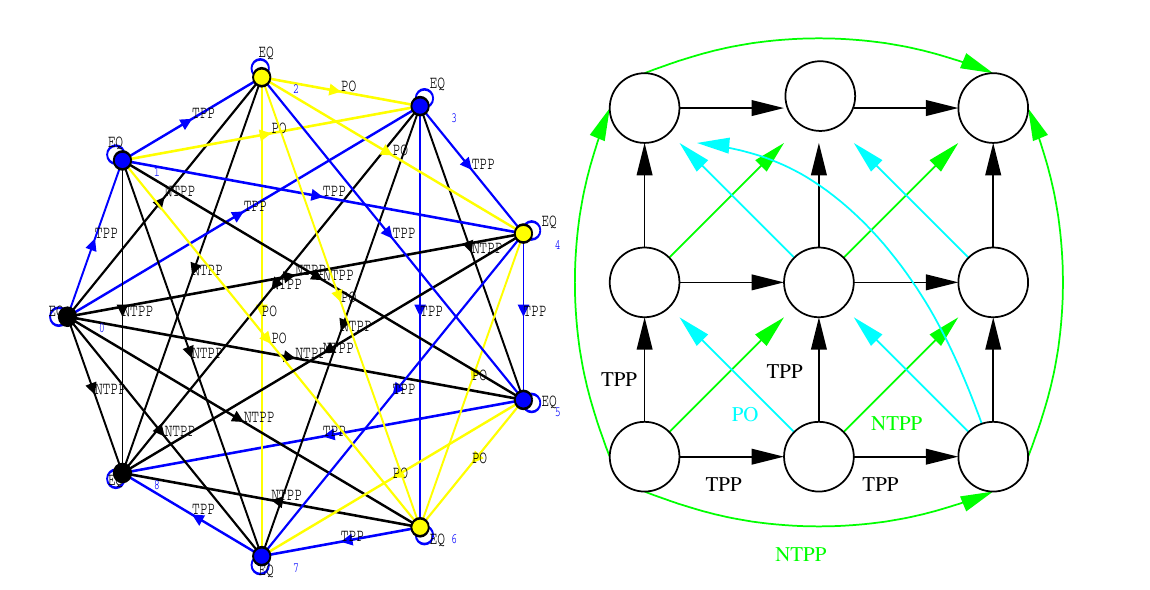
\includegraphics[width=.72\textwidth]{report7_figure10_grid.png}
\end{center}
\vspace{-4pt}
{\small An RCC8 network isomorphic to an $n\times n$ grid (report7,
Fig.~10, 2002/2003) --- the construction \emph{found by a Lisp enumerator}
and drawn with CLIM (MCL), not by hand. The models are \emph{out there}.}
\end{frame}

%% ==================================================================== 15
\begin{frame}{\dots but no concept can \emph{force} them: the coincidence obstruction}
\begin{center}
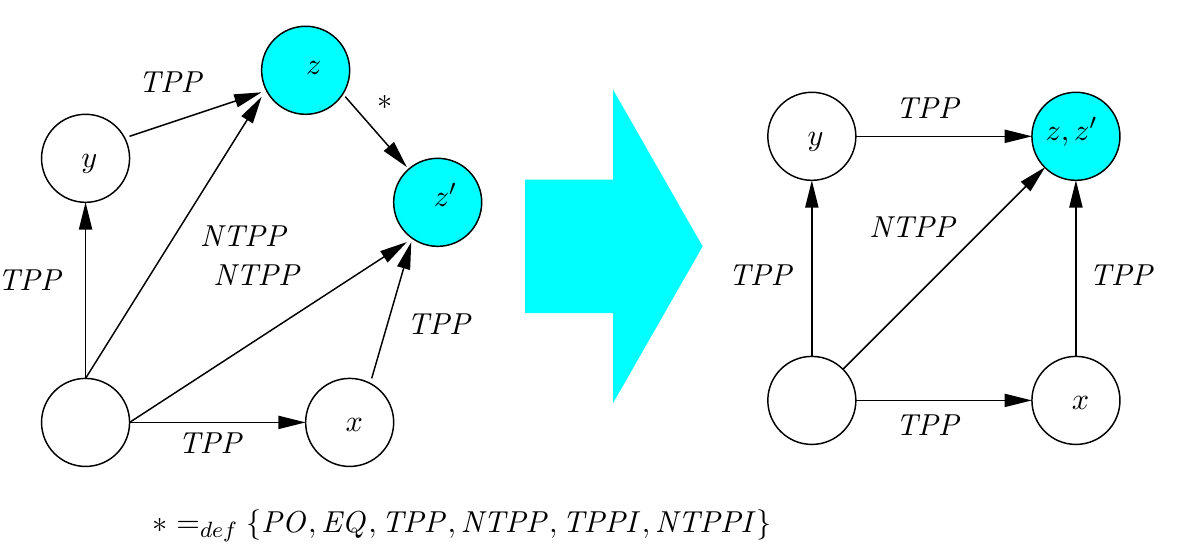
\includegraphics[width=.55\textwidth]{report7_figure11_coincidence.png}
\end{center}
\vspace{-4pt}
{\small report7, Fig.~11: successors $z$ (east-north) and $z'$ (north-east)
\emph{should} be one corner --- the table \emph{alone} allows \alert{six}
relations, forcing neither merge nor split. You \emph{can} force the merge
(clash out the five non-$\EQ$ options, $\EQ$ remains) --- but that's the
trap: those markers collapse \emph{every} corner at the next level (SAT at
level~1, UNSAT at~2; RCC5 \emph{and} RCC8). Neither gives a grid: loose
$\Rightarrow$ no join, forced $\Rightarrow$ total collapse.}
\medskip

\begin{quote}\small
``Even though these infinite models do exist, we have found no way to
\emph{enforce} the depicted model(s) by means of a concept term.''
\hfill (report7, 2003)
\end{quote}
\end{frame}

%% ==================================================================== 16
\section{The 2026 campaign}
\begin{frame}{The cast, and the loop}
\begin{center}
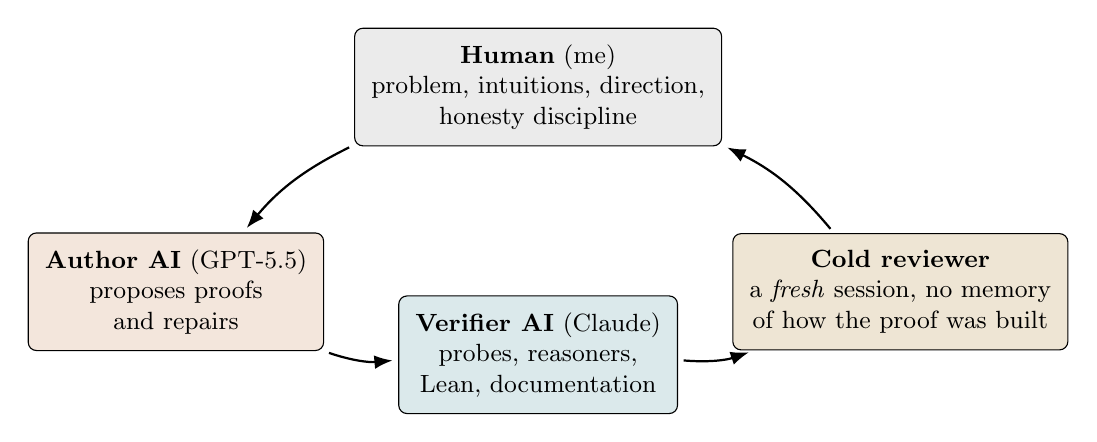
\begin{tikzpicture}[
  n/.style={draw, rounded corners=3pt, align=center, inner sep=6pt, font=\small},
  e/.style={-{Latex}, thick, shorten >=2pt, shorten <=2pt}]
  \node[n, fill=black!8]   (h) at (0,1.7)  {\textbf{Human} (me)\\ problem, intuitions, direction,\\ honesty discipline};
  \node[n, fill=warm!15]   (a) at (-4.6,-.9) {\textbf{Author AI} (GPT-5.5)\\ proposes proofs\\ and repairs};
  \node[n, fill=petrol!15] (v) at (0,-1.7)   {\textbf{Verifier AI} (Claude)\\ probes, reasoners,\\ Lean, documentation};
  \node[n, fill=openc!18]  (r) at (4.6,-.9)  {\textbf{Cold reviewer}\\ a \emph{fresh} session, no memory\\ of how the proof was built};
  \draw[e] (h) to[bend right=12] (a);
  \draw[e] (a) to[bend right=12] (v);
  \draw[e] (v) to[bend right=12] (r);
  \draw[e] (r) to[bend right=12] (h);
\end{tikzpicture}
\end{center}
\vfill
Propose $\to$ verify $\to$ \alert{attack} $\to$ repair. Round after round,
March--July 2026.
\end{frame}

%% ==================================================================== 17
\begin{frame}{The campaign at a glance}
\begin{columns}[T]
\column{.48\textwidth}
\begin{itemize}
  \item $\sim$4 months, $\sim$\alert{30 repair rounds}
  \item \alert{17 adversarial reviews} --- a defect or overclaim found in
        \emph{all but two}
  \item \alert{88} self-contained verification probes (each re-derives the
        algebra from set semantics)
  \item 4 Lean files, $\sim$\alert{5{,}900 lines}, \alert{zero \texttt{sorry}}
  \item 2 working reasoners, cross-validated on \alert{911 concepts}
\end{itemize}
\column{.48\textwidth}
\begin{block}{The single most telling number}
  Across \emph{all} rounds and reviews,
  \alert{no accepted-but-unsatisfiable concept was ever found}.
  Every defect was a gap in an \emph{argument} ---
  never a counterexample to the intended theorem.
\end{block}
\medskip
{\small That is why the label is \emph{strongly supported} --- and why it is
still \emph{not certified}.}
\end{columns}
\end{frame}

%% ==================================================================== 18
\begin{frame}{Route 1: tableaux with blocking --- broken by totality}
The default DL method: build a model top-down, \emph{block} when a node
repeats an ancestor's type.
\vfill
\begin{itemize}
  \item Here, composition forces edges \alert{into already-built nodes}:
        from $x\,\PP\,y$, $y\,\DR\,z$ the table forces $x\,\DR\,z$.
  \item Diagnostic: \;
        $C_{\mathrm{force}}=\exists\PP.(\exists\DR.A)\sqcap\forall\DR.\neg A$
        \; is \textbf{unsatisfiable} --- any procedure that ignores forced
        edges wrongly accepts it.
  \item Dormant $\forall$'s reawaken blocked nodes; no fixed-arity local
        summary (types, triangles, quadruples, profiles, \dots) is ever enough.
\end{itemize}
\vfill
\begin{center}
\alert{Lesson: in a total-relation logic, ``local'' does not exist.}\\
What may be reused depends on the whole graph. (That is F6 in disguise.)
\end{center}
\end{frame}

%% ==================================================================== 19
\begin{frame}{Route 2: the split-forest idea (a whiteboard, April 2026)}
\begin{columns}[T]
\column{.5\textwidth}
  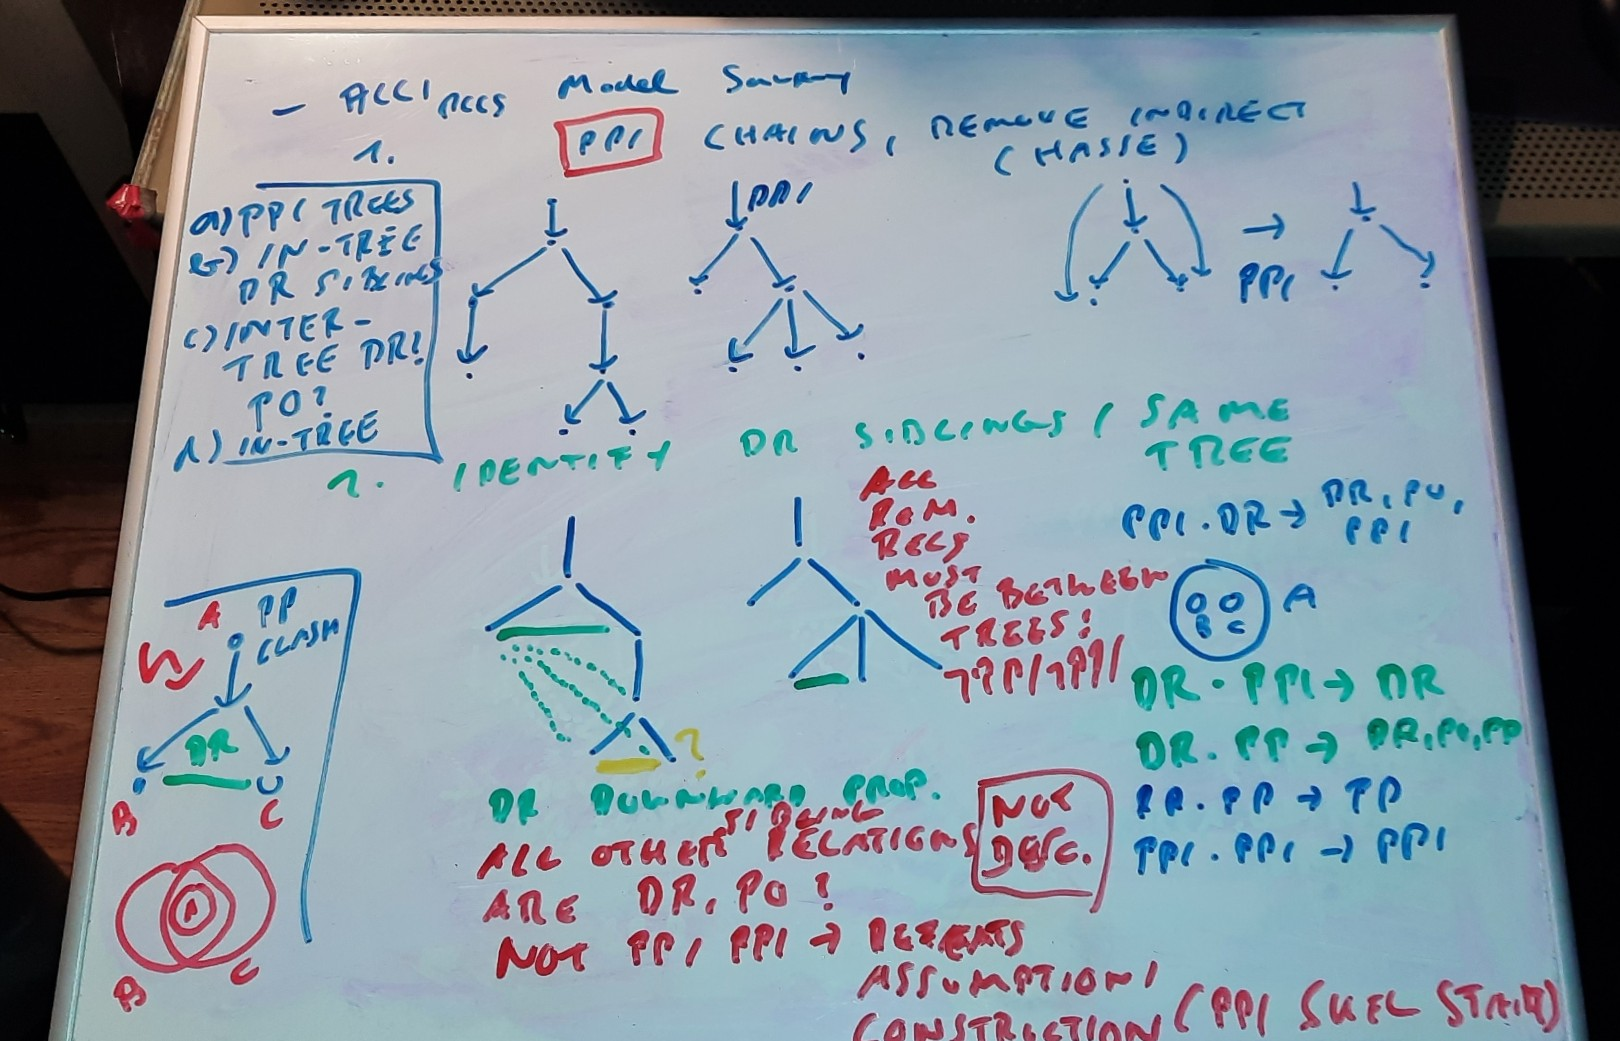
\includegraphics[width=\textwidth]{20260407_062616.jpg}
\column{.46\textwidth}
  \begin{itemize}
    \item \alert{Present} the complete graph as a \emph{forest of part-of trees}:
          split shared parts into $\EQ$-mates, re-orient vertical edges into
          the trees.
    \item All remaining cross-edges are \alert{horizontal}; complete them by
          the RCC5 \emph{patchwork property} (a citable classical theorem).
    \item The one component \alert{every} cold review found sound ---
          the semantic foundation all later routes consume.
  \end{itemize}
\end{columns}
\vfill
{\small The human contribution: this decomposition. The models made it precise.}
\end{frame}

%% ==================================================================== 20
\begin{frame}{Route 3: tree automata --- ``acceptance without validity''}
Package the search as a parity tree automaton (emptiness is decidable)\dots
\vfill
\begin{itemize}
  \item \dots but the input tree \alert{omits} the relations between fresh
        witnesses and the sources of $\forall$-constraints.
  \item An \emph{alternating} automaton explores in independent copies ---
        and copies \alert{guess the missing relations independently}.
  \item A cold review built the killer: two copies privately guess
        $\{\PP\}$ and $\{\DR\}$ for the same pair;
        $\comp(\PP,\PP)\cap\comp(\PP,\DR)=\{\PP\}\cap\{\DR\}=\emptyset$
        --- every copy accepts, \alert{no model exists}.
\end{itemize}
\vfill
\begin{center}
So the automaton was \alert{abandoned}, in favour of explicit finite
certificates checked by composition tests --- with a \emph{truth lemma}
instead of an acceptance condition. (This is what got formalized.)
\end{center}
\end{frame}

%% ==================================================================== 21
\section{What we actually got}
\begin{frame}{Machine-checking: what the Lean kernel buys}
\begin{columns}[T]
\column{.52\textwidth}
  \begin{itemize}
    \item \alert{Lean 4}: a proof assistant whose kernel type-checks
          \emph{every} inference; a proof with a gap \emph{does not compile}.
    \item Our discipline: Lean 4 \alert{core only} --- no libraries; every
          object built from first principles; tiny trusted base.
    \item ``\alert{zero \texttt{sorry}}'' = no admitted gaps anywhere.
  \end{itemize}
\column{.44\textwidth}
  \begin{block}{Why we moved to Lean}
    Most reviews broke a \emph{prose} proof --- typically at a
    step that was \emph{assumed}, not proved. The kernel cannot be talked
    past. After the move, reviews stopped finding soundness defects and
    started finding only \emph{interface} gaps --- which were then closed.
  \end{block}
\end{columns}
\end{frame}

%% ==================================================================== 22
\begin{frame}{What exactly is certified (zero \texttt{sorry})}
\begin{center}
\scriptsize
\begin{tabular}{lll}
\toprule
Result & Meaning & File\\
\midrule
\textcolor{good}{\textbf{Soundness pipeline}} &
  valid certificate $\Rightarrow$ real RCC5 model &
  \texttt{Round19Transport}\\
\textcolor{good}{\textbf{Abstraction faithful}} &
  satisfiable $\Leftrightarrow$ Hintikka-realizable &
  \texttt{Round19Transport}\\
\textcolor{good}{\textbf{RCC5 normal form}} (both dir.) &
  network $\Leftrightarrow$ order + disjointness &
  \texttt{RCC5NormalForm}\\
\textcolor{good}{\textbf{Forcing reduction}} &
  F6 fails $\Leftrightarrow$ a concept forces crowds &
  \texttt{ForcingReduction}\\
\textcolor{good}{\textbf{Dovetail schema}} &
  qualitative F6 $\Rightarrow$ decidable &
  \texttt{SemiDecidability}\\
\bottomrule
\end{tabular}
\end{center}
\vfill
What is \alert{deliberately not} in the kernel: the open completeness
premise itself (F6). It is \emph{stated}, never axiomatized --- the honest
boundary between what is proved and what is conjectured.
\end{frame}

%% ==================================================================== 23
\begin{frame}{The main theorem (conditional, soundness certified)}
\begin{block}{Conditional decidability}
  \textbf{If} F6 holds --- live width bounded by a computable function of
  the concept --- \textbf{then} $\ALCIRCC{5}$ concept satisfiability is
  \alert{decidable}.
\end{block}
\vfill
\begin{itemize}
  \item The \alert{soundness half} is kernel-checked end to end:
        certificate syntax $\to$ closure conditions $\to$ proper RCC5 frame
        $\to$ truth lemma $\to$ \emph{actual model of the input concept}.
  \item The certificate checker is a real \alert{executable Boolean function}
        --- no oracle anywhere (a previous version had a hidden one;
        a cold review caught it; it was rebuilt).
  \item Everything that remains open is the \alert{antecedent} --- F6.
\end{itemize}
\end{frame}

%% ==================================================================== 24
\begin{frame}{Unconditional win \#1: a decidable fragment}
\begin{block}{Theorem ($\forall\PO$-free fragment)}
  Concepts with \alert{no $\forall\PO$ subformula} are decidable, with
  live width $\leq (1+m)^2\, 2^{2^m}$, \; $m = |\cl(C_0)|$.
\end{block}
\vfill
\begin{itemize}
  \item Still allowed: $\exists\PO$ (``overlaps some\dots''),
        $\forall\DR$, $\exists\DR$, and \alert{all} part-of modalities ---
        a genuinely expressive spatial fragment.
  \item Why it works: $\PO$ is the \emph{only} relation whose recurrence
        along a chain needs an ``all-phase'' safety condition; drop
        $\forall\PO$ and the condition is vacuous.
  \item Found twice, independently, by two different routes --- a good sign
        the fragment is natural, not an artifact.
\end{itemize}
\end{frame}

%% ==================================================================== 25
\begin{frame}{Unconditional win \#2: the RCC5 normal form}
\begin{block}{Theorem (both directions kernel-checked, arbitrary domains)}
  A strong-$\EQ$ RCC5 network is composition-closed \emph{iff} it is an
  \alert{ordered-disjoint structure}:
  \begin{itemize}
    \item $\PP$ is a strict partial order (a genuine part-of hierarchy);
    \item $\DR$ is a symmetric, \alert{downward-closed} disjointness;
    \item comparable pairs never disjoint; $\PO$ is the residual.
  \end{itemize}
\end{block}
\vfill
Every RCC5 model, anywhere, \emph{is} just: a hierarchy + a
downward-inherited ``keeps-apart'' relation + overlap as the leftover.
The ``$\Rightarrow$'' is a 150-line kernel proof (\texttt{propext} only);
the ``$\Leftarrow$'' is GPT-5.6~Pro's \alert{canonical set representation},
also kernel-checked for arbitrary domains --- the structural fact both major
proof routes silently relied on, now a certified biconditional.
\end{frame}

%% ==================================================================== 26
\begin{frame}{A late surprise: the problem's exact address is $\Pi^0_1$}
\begin{columns}[T]
\column{.54\textwidth}
\begin{center}
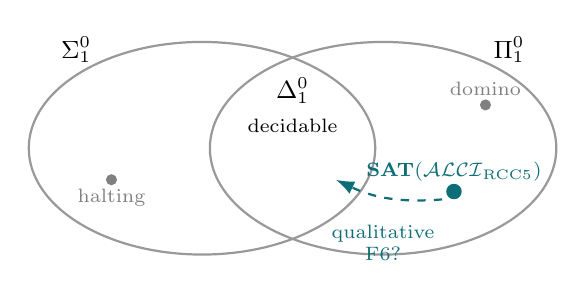
\begin{tikzpicture}[scale=1.0]
  \draw[thick,black!40] (-1.15,0) ellipse (2.2 and 1.35);
  \draw[thick,black!40] (1.15,0) ellipse (2.2 and 1.35);
  \node at (-2.75,1.25) {\small $\Sigma^0_1$};
  \node at (2.75,1.25) {\small $\Pi^0_1$};
  \node[align=center] at (0,.55) {\small $\Delta^0_1$\\ \scriptsize decidable};
  \fill[black!50] (-2.3,-.4) circle (2pt) node[below,font=\scriptsize] {halting};
  \fill[black!50] (2.45,.55) circle (2pt) node[above,font=\scriptsize] {domino};
  \fill[petrol] (2.05,-.55) circle (2.8pt)
     node[above,font=\scriptsize,petrol] {\textbf{SAT}$(\ALCIRCC{5})$};
  \draw[-{Latex}, dashed, petrol, thick] (1.9,-.65) to[bend left=15] (.55,-.4);
  \node[petrol,font=\scriptsize,align=center] at (1.15,-1.2) {qualitative\\ F6?};
\end{tikzpicture}
\end{center}
\column{.44\textwidth}
\begin{itemize}
  \item The whole semantics is \alert{finitely first-order axiomatizable};
        by G\"odel completeness, \emph{un}satisfiability is enumerable.
  \item So SAT is \alert{co-r.e.} ($\Pi^0_1$) --- the domino problem's
        \emph{ceiling} (membership; we don't claim hardness).
  \item Nobody in the project --- or the reviews --- had noticed for four
        months. Machine-cross-checked; the reduction is in Lean.
\end{itemize}
\end{columns}
\end{frame}

%% ==================================================================== 27
\begin{frame}{Consequence: half of the keystone was never needed}
A $\Pi^0_1$ problem is decidable \emph{iff} SAT is also enumerable. So run
\alert{two search parties} and wait for the first hit:
\begin{center}
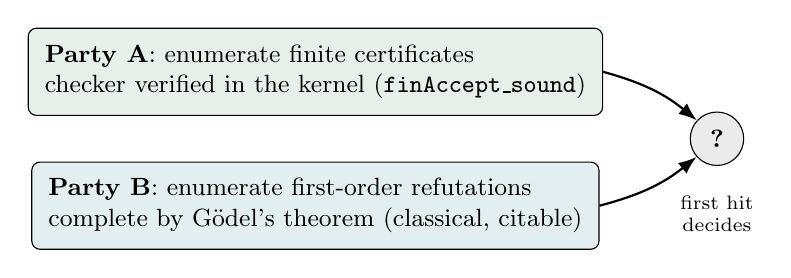
\begin{tikzpicture}[font=\small,
  lane/.style={draw, rounded corners=3pt, align=left, inner sep=6pt}]
  \node[lane, fill=good!12]  (a) at (0,0.85)
    {\textbf{Party A}: enumerate finite certificates\\
     checker verified in the kernel (\texttt{finAccept\_sound})};
  \node[lane, fill=petrol!12] (b) at (0,-0.85)
    {\textbf{Party B}: enumerate first-order refutations\\
     complete by G\"odel's theorem (classical, citable)};
  \node[draw, circle, fill=black!8, inner sep=4pt] (w) at (5.1,0) {\textbf{?}};
  \draw[-{Latex},thick] (a.east) to[bend left=12] (w);
  \draw[-{Latex},thick] (b.east) to[bend right=12] (w);
  \node[font=\scriptsize, align=center] at (5.1,-.95) {first hit\\ decides};
\end{tikzpicture}
\end{center}
\begin{itemize}
  \item Needed now: only \alert{qualitative} F6 --- \emph{some} finite
        certificate per satisfiable concept, \alert{no computable bound}.
  \item The bound the reviewers kept demanding (and that kept breaking)
        comes back \alert{for free, afterwards} --- a theorem of the schema.
\end{itemize}
\end{frame}

%% ==================================================================== 28
\begin{frame}{``Isn't this just first-order logic?'' --- yes, and it helps}
$\ALCIRCC{5}$-SAT \emph{is} FO satisfiability of a finite theory. Does it
land in a \alert{decidable fragment} of FO?
\begin{center}
\small
\begin{tabular}{lll}
\toprule
Fragment & Fate & Why\\
\midrule
two-variable FO$^2$ & \xmark & composition is ternary
   \hfill {\footnotesize(RCC3 \emph{did} fall this way in 2003!)}\\
prefix classes & \xmark & unbounded $\forall\exists$ alternation, FMP\\
guarded / clique-guarded & \xmark & \alert{totality} is the one unguardable axiom\\
unary/guarded negation & \xmark & finite model property; totality again\\
guarded + transitivity & \xmark & undecidable outside guards\\
\bottomrule
\end{tabular}
\end{center}
\vfill
Every failure traces to the same fact: \alert{every pair is related}, so
models are maximally non-local --- exactly the obstruction F6 names.
The FO view rediscovers the project's wall from classical model theory.
\end{frame}

%% ==================================================================== 29
\section{The reasoner: a 23-year loop closed}
\begin{frame}{A working prototype reasoner (validated, not proved)}
\begin{itemize}
  \item The \alert{cover-tree tableau} ($\sim$350 lines of Python):
        exact-occurrence blocking on the split-forest foundation.
  \item Cross-validated against an independent oracle on
        \alert{911 concepts --- zero mismatches}; $775/775$ structured
        decomposition tests; never once contradicted in the whole campaign.
  \item Decides correctly even the known trap (the strong-$\EQ$ $\PO$-loop)
        that fools type-based procedures.
\end{itemize}
\vfill
\begin{center}
A running algorithm and a kernel-checked proof, \alert{pointing the same
way} --- the strongest evidence short of a certificate.
\end{center}
\end{frame}

%% ==================================================================== 30
\begin{frame}{2003: a prototype reasoner}
\begin{center}
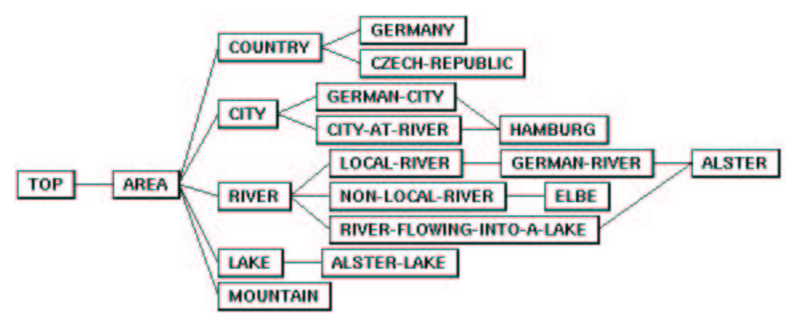
\includegraphics[height=.72\textheight]{report7_figure6_taxonomy.png}
\end{center}
\vspace{-4pt}
{\small The GIS concept taxonomy in report7 (Fig.~6), 2003 --- itself
\emph{computed by a prototype reasoner} of the era, not drawn by hand.}
\end{frame}

%% ==================================================================== 31
\begin{frame}{2026, the cover-tree reasoner: all 21/21 --- edge for edge}
\begin{center}
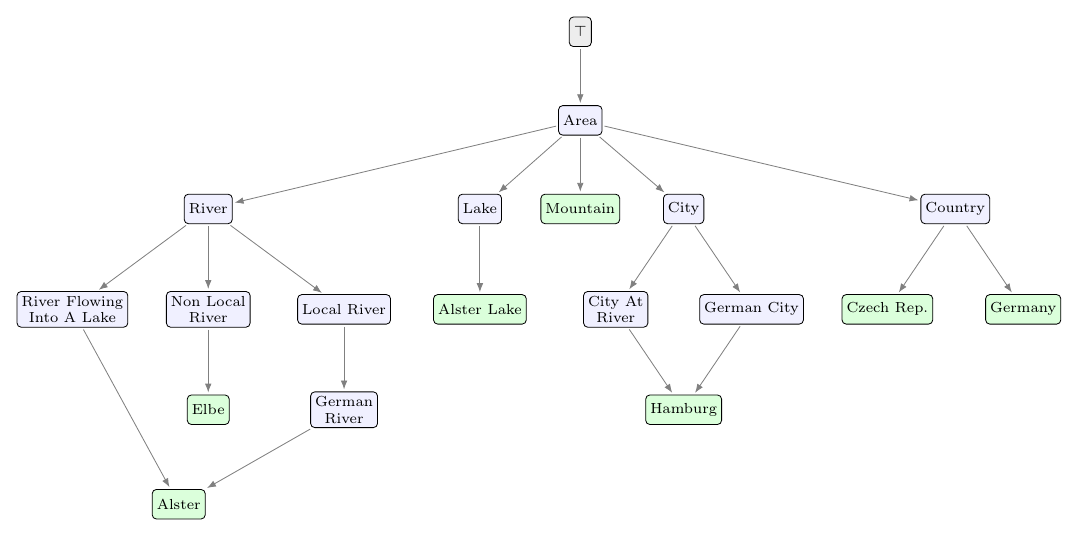
\includegraphics[width=.82\textwidth]{gis_taxonomy_reasoner_2026.png}
\end{center}
\vspace{-2pt}
{\small The 2026 cover-tree tableau reproduces it exactly --- \alert{two
reasoners, 23 years apart, identical result}. (Green = individuals;
\emph{Hamburg} and \emph{Alster} each have \alert{two} parents --- a DAG,
not a tree.)}
\end{frame}

%% ==================================================================== 32
\section{Lessons: working with frontier AI}
\begin{frame}{What the models did --- and what they could not}
\begin{columns}[T]
\column{.48\textwidth}
\textbf{\textcolor{good}{Demonstrated}}
\begin{itemize}
  \item months-long rigorous formal development, $\sim$30 rounds
  \item genuinely useful \emph{adversarial} review (with machine-checked witnesses)
  \item a 5{,}900-line kernel-checked Lean development
  \item working, validated software
\end{itemize}
\column{.48\textwidth}
\textbf{\textcolor{openc}{Not demonstrated}}
\begin{itemize}
  \item the \alert{decisive novel idea} --- F6 is uncracked
  \item reliable \emph{self}-review (both models declared victory prematurely; both were caught)
  \item working unsupervised: the human directed every round
\end{itemize}
\end{columns}
\vfill
\begin{center}
Neither model is self-sufficient. \alert{What carried the project was the loop, not any single model.}
\end{center}
\end{frame}

%% ==================================================================== 33
\begin{frame}{The method that worked (steal this)}
\begin{enumerate}
  \item \textbf{Cold review beats hot review.} A \emph{fresh} session with no
        memory of the construction found what warm reviewers missed ---
        every time it mattered. Make it a standard step.
  \item \textbf{Don't trust --- verify.} Every load-bearing claim was
        cross-checked mechanically: 88 probes that re-derive the algebra
        from set semantics, and ultimately the Lean kernel. The machine
        checks are the ground truth, \alert{not the model's confidence}.
  \item \textbf{Label honestly.} \emph{Strongly supported} $\neq$
        \emph{certified}. Overclaiming happened twice; cold review caught
        both; the claims were withdrawn --- \alert{on the record}.
\end{enumerate}
\vfill
{\small The full timestamped conversation log is public --- every idea,
defect, and repair traceable to its origin, human or model.}
\end{frame}

%% ==================================================================== 34
\begin{frame}{If nothing else: a message to fellow researchers}
\begin{itemize}
  \item Whatever the fate of the mathematics, this campaign is an
        \alert{existence proof} of what frontier models could already do in
        serious formal research --- \emph{in July 2026}.
  \item Anyone doing serious logic or mathematics should \alert{know} these
        capabilities exist. Ignoring them does not advance science;
        declining to use them is simply unwise.
  \item Saying exactly this was a stated purpose of the work. Its first
        outing (DL 2026) was rejected without engaging either the
        mathematics or the message --- so it is now on arXiv,
        \alert{in the open}, with the full audit trail.
\end{itemize}
\vfill
\begin{center}
\emph{The instruments have changed. The standards --- verification,
adversarial review, honest labels --- matter more than ever.}
\end{center}
\end{frame}

%% ==================================================================== 34b
\begin{frame}{The results, by verification level}
\begin{center}
\scriptsize
\renewcommand{\arraystretch}{1.15}
\begin{tabular}{@{}p{2.3cm}p{6.1cm}p{2.6cm}@{}}
\toprule
\textbf{Level} & \textbf{Results} & \textbf{What it means}\\
\midrule
\textcolor{good}{\textbf{Lean-certified}} &
  soundness pipeline; abstraction faithfulness; RCC5 normal form (both
  directions); $\forall\PO$-free lift core; F6\,$\Rightarrow$\,decidable;
  $\Pi^0_1$ dovetail &
  kernel-checked, with a stated axiom footprint\\
\addlinespace
\textbf{Theorem-level} &
  $\forall\PO$-free decidability + bound; identity-selector
  characterization; W2$'$ folds into F6 &
  proof in a work package, often with probes\\
\addlinespace
\textbf{Empirical} &
  cover-tree tableau; 911-concept cross-validation; model verifier &
  test evidence, not a decision theorem\\
\addlinespace
\textcolor{openc}{\textbf{Open}} &
  static F6; completeness of the certificate scheme; automatic-cover
  property; full decidability &
  no proof claimed\\
\bottomrule
\end{tabular}
\end{center}
\vfill
{\small Four levels kept rigorously distinct --- conflating them is the
easiest way to misread the project.}
\end{frame}

%% ==================================================================== 35
\begin{frame}{Where it stands}
\begin{center}
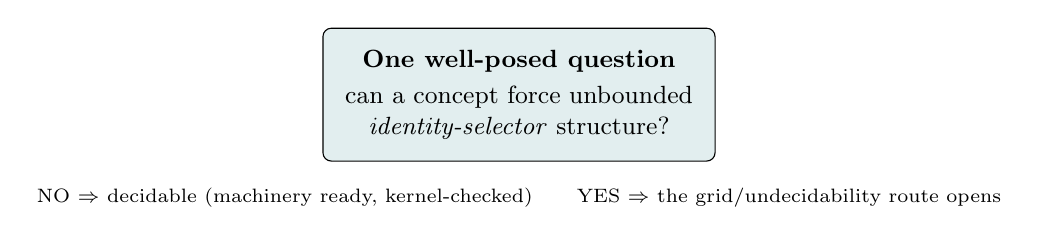
\begin{tikzpicture}[font=\small]
  \node[draw, rounded corners=3pt, fill=petrol!12, inner sep=8pt, align=center] (q)
    {\textbf{One well-posed question}\\[2pt]
     can a concept force unbounded\\ \emph{identity-selector} structure?};
  \node[below=6pt of q, align=center, font=\scriptsize]
    {NO $\Rightarrow$ decidable (machinery ready, kernel-checked)\qquad
     YES $\Rightarrow$ the grid/undecidability route opens};
\end{tikzpicture}
\end{center}
\vfill
\begin{itemize}
  \item 20+ years of difficulty, compressed into one lemma --- with certified
        machinery waiting on \alert{both} sides of the answer.
  \item Everything is frozen, tagged, reproducible: paper (42pp), 4 Lean
        files, 88 probes, 2 reasoners, full conversation log.
\end{itemize}
\vfill
\begin{center}
  \alert{\textbf{Open since 2003. Smaller than ever. Still standing.}}\\[4pt]
  \small\texttt{github.com/lambdamikel/alcircc5} \quad---\quad thank you!
\end{center}
\end{frame}

%% ==================================================================== backup
\appendix
\begin{frame}{Backup: the full RCC5 composition table}
\begin{center}
\renewcommand{\arraystretch}{1.2}
\small
\begin{tabular}{l|ccccc}
\toprule
$\comp$ & $\DR(a,b)$ & $\PO(a,b)$ & $\EQ(a,b)$ & $\PPI(a,b)$ & $\PP(a,b)$ \\
\midrule
$\DR(b,c)$ & $*$ & $\DR,\PO,\PPI$ & $\DR$ & $\DR,\PO,\PPI$ & $\DR$ \\
$\PO(b,c)$ & $\DR,\PO,\PP$ & $*$ & $\PO$ & $\PO,\PPI$ & $\DR,\PO,\PP$ \\
$\EQ(b,c)$ & $\DR$ & $\PO$ & $\EQ$ & $\PPI$ & $\PP$ \\
$\PP(b,c)$ & $\DR,\PO,\PP$ & $\PO,\PP$ & $\PP$ & $\PO,\EQ,\PP,\PPI$ & $\PP$ \\
$\PPI(b,c)$ & $\DR$ & $\DR,\PO,\PPI$ & $\PPI$ & $\PPI$ & $*$ \\
\bottomrule
\end{tabular}
\end{center}
\vfill
{\small Row = $S(b,c)$, column = $R(a,b)$, entry = possibilities for
$(a,c)$; $*$ = all five. Re-derived from finite set semantics by every
probe; matches the certified Lean table cell for cell.}
\end{frame}

\begin{frame}{Backup: what a finite certificate looks like}
\begin{itemize}
  \item \textbf{Catalogue} (the finite blueprint):
    \begin{itemize}
      \item a \emph{core network} --- the non-repeating part of the model;
      \item finitely many \emph{attachment templates} --- recipes for gluing a
            fresh witness cluster onto an interface;
      \item a \emph{steering function} fixing the horizontal relations from
            old occurrences to fresh ones (the only real freedom).
    \end{itemize}
  \item \textbf{Plan}: which template to apply where; \emph{unfolding} it
        (possibly forever) produces the split-forest model.
  \item \textbf{Soundness}, kernel-checked: one finite check on the catalogue
        guarantees \emph{every} unfolding is a legal RCC5 model.
  \item \textbf{Live width} = live occurrences that must coexist at one
        interface during unfolding --- the quantity F6 must bound.
\end{itemize}
\end{frame}

\begin{frame}{Backup: the sharpened F6 --- identity-selector minors}
\begin{itemize}
  \item The naive ways to force width (shell half-graphs, prefix pumps,
        $\PO$-gaps) all \alert{collapse} to finite catalogues --- machine-checked.
  \item The sharp obstruction: $n$ pairs $(L_i, U_i)$, each kept apart by a
        \alert{private} selector $A_i$ and by nothing else --- the selector
        incidence matrix is the $n\times n$ \emph{identity}.
  \item A finite catalogue can hold only boundedly many private selectors,
        so: \textbf{F6 fails iff some concept forces such minors for every $n$.}
  \item Bare RCC5 networks with unbounded such structure \emph{exist}
        (machine-checked) --- so any F6 proof must use
        \emph{$\ALCIRCC{}$-forceability}, not RCC5 consistency alone.
        The uniformization side-condition (W2$'$) provably folds into F6.
\end{itemize}
\end{frame}

\end{document}
